\documentclass[11pt]{article}
\usepackage[margin=0.9in]{geometry}
\usepackage{graphicx}
\usepackage{booktabs}
\usepackage{amsmath}
\usepackage[font=small,labelfont=bf]{caption}
\usepackage{xcolor}
\usepackage{eurosym}
\usepackage{enumitem}
\PassOptionsToPackage{hyphens}{url}
\usepackage[hidelinks]{hyperref}
\newcommand{\todo}[1]{\textcolor{red}{[#1]}}
\setlength{\parskip}{0.4em}
\setlength{\parindent}{0pt}
\setlist{nosep, leftmargin=1.5em}
\renewcommand{\topfraction}{0.9}
\renewcommand{\bottomfraction}{0.8}
\renewcommand{\textfraction}{0.07}
\renewcommand{\floatpagefraction}{0.85}
\setcounter{topnumber}{3}
\setcounter{totalnumber}{4}

\title{STATS525 Progress Report:\\ Soccer players' market value}
\author{Hugh Koschwanez, Omar Haque, Raj Patel}
\date{November 12, 2026}

\begin{document}
\maketitle

\textbf{Research question.} Which player characteristics are associated with a soccer player's market value? Our predictors are age, goals plus assists per 90 minutes (G+A/90), pass completion (\%), minutes played and position (DF, MF, FW, GK).

\textbf{Data.} The Kaggle data set ``Soccer players values and their statistics''~[1] combines market values in euros from transfermarkt.de with player statistics from fbref.com. We use the 2017/18 season.

\section*{Part A: Data exploration and initial modeling}

\subsection*{A.1 Data cleaning}
Starting from 2{,}231 players, we:
\begin{itemize}
    \item multiplied the 349 market values below \euro1M by 10. No player was valued between \euro90{,}000 and \euro1M, which points to a scraping error (Transfermarkt lists these values in thousands, e.g.\ ``900 Tsd.~\euro''). The correction fills the gap (Figure~\ref{fig:dist}, third panel);
    \item removed 14 rows where two different players share a name and were given the same value;
    \item merged 107 players listed twice because they changed clubs during the season;
    \item kept only the first listed position (e.g.\ ``FW,MF'' becomes FW);
    \item removed 471 players with fewer than 450 minutes (five full games), whose per-90 statistics are unreliable, and one player with missing passing data.
\end{itemize}
The final data set has \textbf{1{,}638 players}: 614 DF, 527 MF, 384 FW and 113 GK.

\subsection*{A.2 Distributions}
Market value is strongly right-skewed: the median is \euro5.0M, the mean \euro11.6M and the maximum \euro180M (Figure~\ref{fig:dist}). After taking logs the distribution is roughly symmetric. Age is roughly symmetric (mean 25.9 years). G+A/90 is right-skewed (median 0.12), and a quarter of players have none. Pass completion is left-skewed (mean 75.7\%), with goalkeepers at the low end. Minutes are spread fairly evenly from 450 to 3{,}420.

\begin{figure}[!htb]
    \centering
    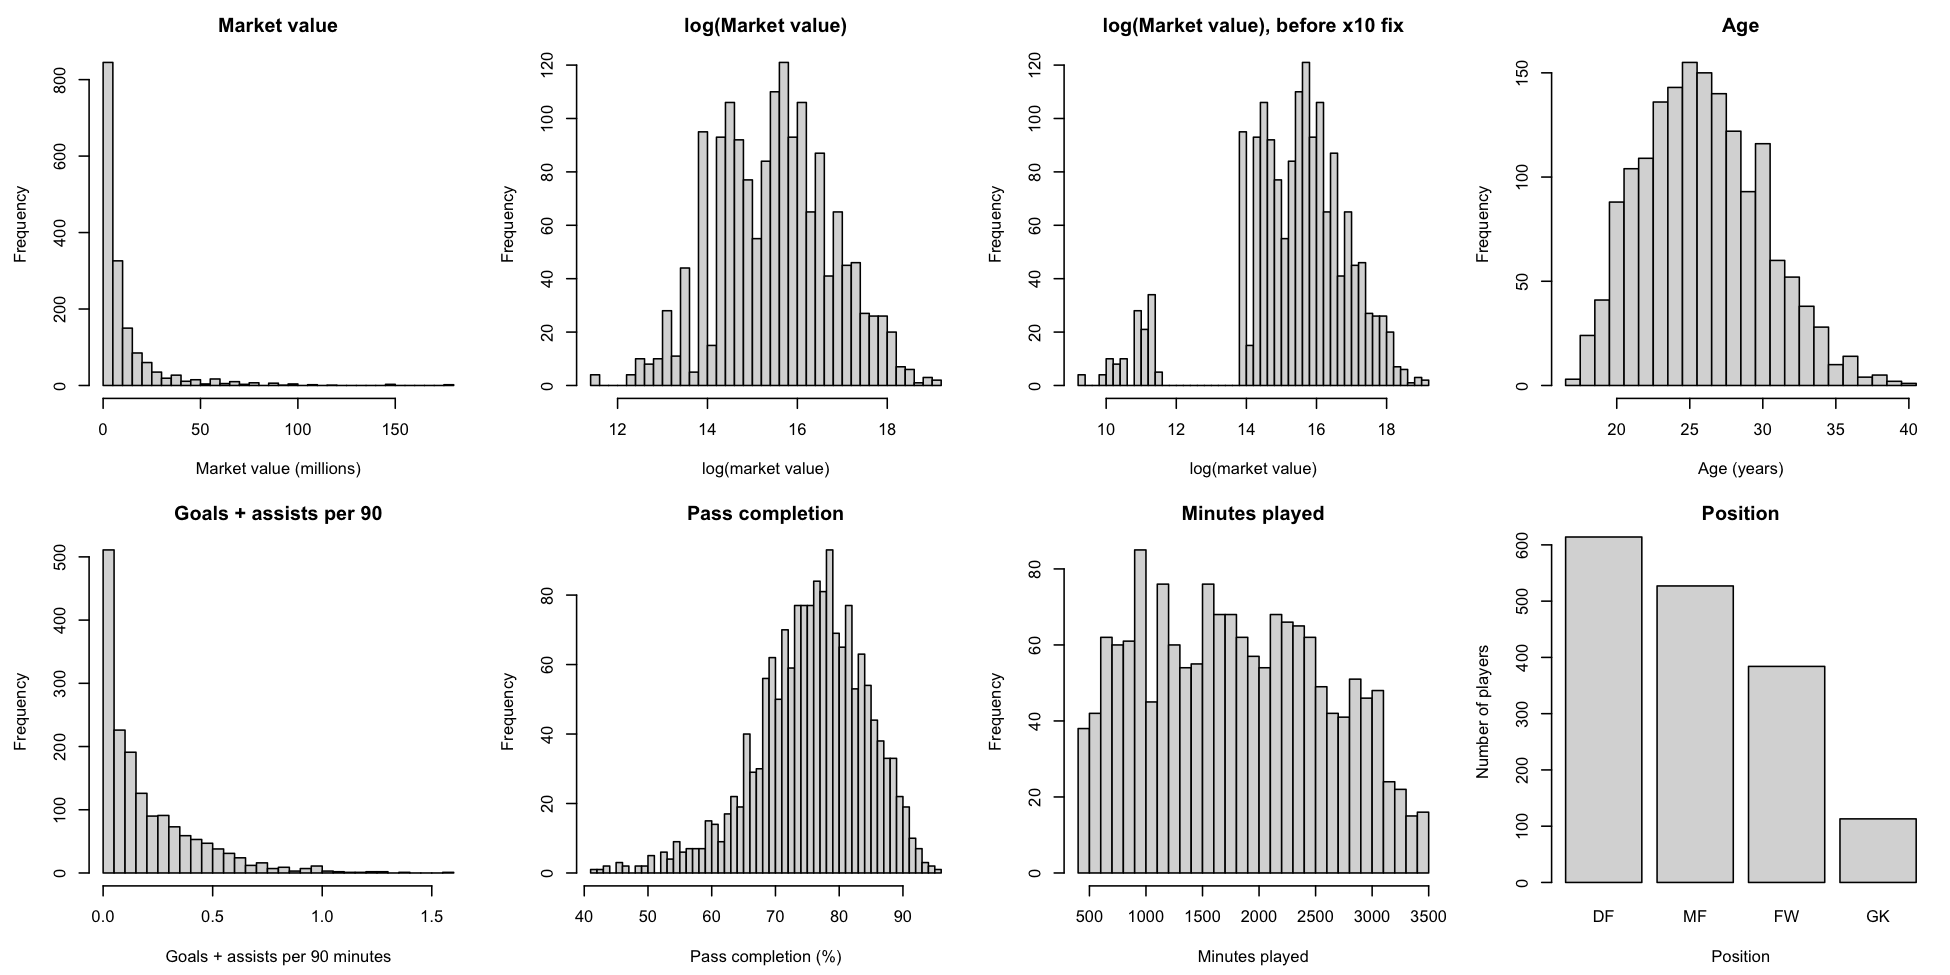
\includegraphics[width=0.92\textwidth]{images/fig1_distributions.png}
    \caption{Histograms of market value, log(market value) after and before the $\times10$ correction, and each predictor, plus the number of players by position ($n = 1{,}638$).}
    \label{fig:dist}
\end{figure}

\subsection*{A.3 Market value versus each predictor}
Market value increases with G+A/90 and with minutes played, and weakly with pass completion (Figure~\ref{fig:scatter}). It is highest for players in their early twenties (median \euro7.5M for ages 20--24) and drops sharply after 30. The spread of values grows as values increase. Forwards have the highest median value (\euro7.0M) and goalkeepers the lowest (\euro4.0M).

\begin{figure}[!htb]
    \centering
    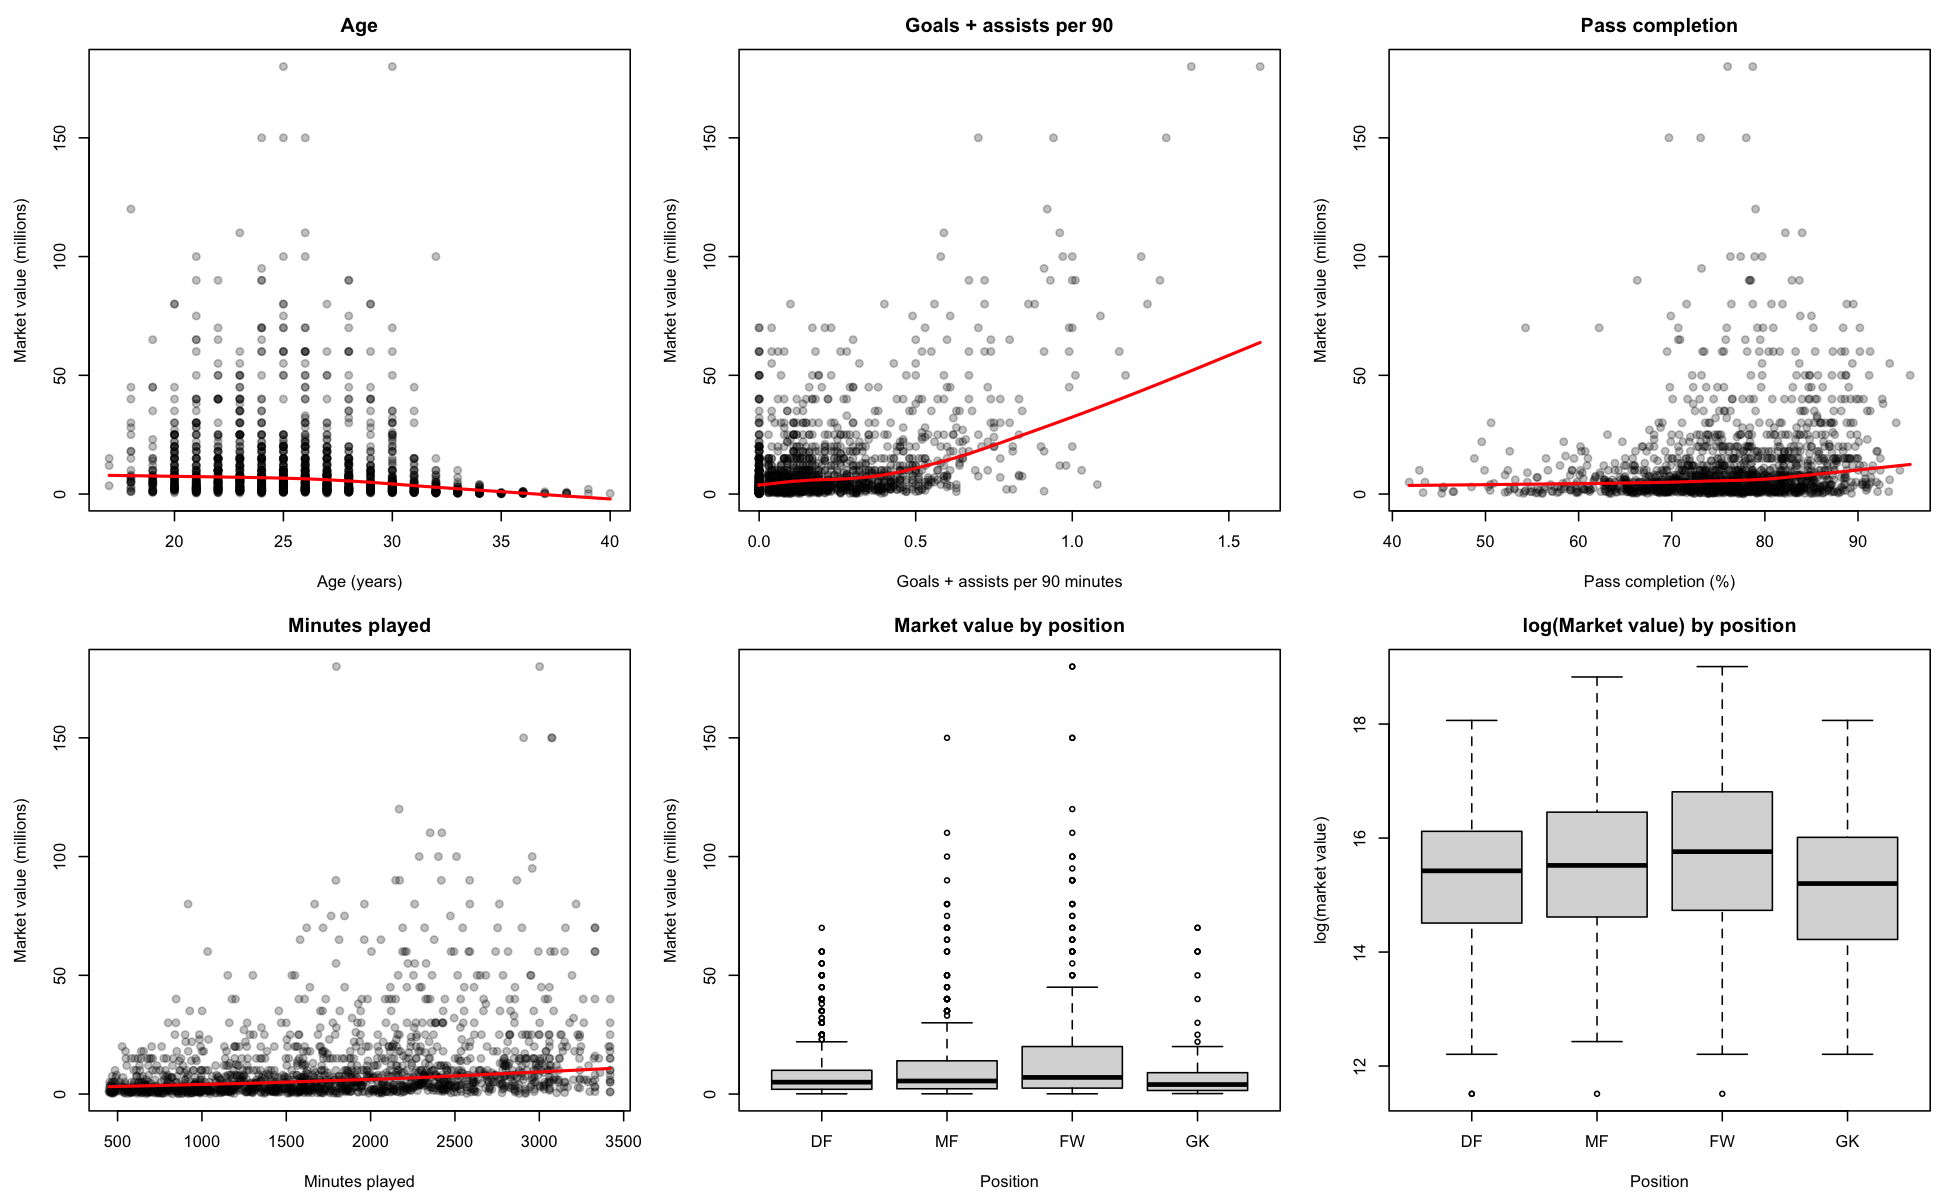
\includegraphics[width=0.78\textwidth]{images/fig2_scatterplots.png}
    \caption{Market value (millions) against each quantitative predictor with a smooth trend line (red), and boxplots of market value by position on the raw and log scales.}
    \label{fig:scatter}
\end{figure}

\subsection*{A.4 Outliers and extreme values}
By the boxplot rule (above $Q_3 + 1.5\,\mathrm{IQR}$), 164 players have unusually high values. The 12 most valuable (\euro100M or more) are stars such as Lionel Messi and Neymar (\euro180M each). These values are real, so we keep them; on the log scale they are no longer extreme. The data errors we found were handled in A.1.

\subsection*{A.5 Transformations}
A Box-Cox analysis gives $\hat\lambda = 0$ (95\% CI $-0.03$ to $0.025$; Figure~\ref{fig:boxcox}), which points to a log transformation of market value. On the log scale, residuals plotted against age and against pass completion are curved (Figure~\ref{fig:diag}, second column), so we also add age$^2$ and (pass \%)$^2$. We subtract each variable's mean before squaring (centering) so that a variable and its square are not highly correlated.

\subsection*{A.6 Correlation among predictors}
The four quantitative predictors are nearly uncorrelated (all $|r| \le 0.09$; Table~\ref{tab:cor}). All variance inflation factors in the final model are below 2.3, so multicollinearity is not a problem.

\begin{figure}[!htb]
    \centering
    \begin{minipage}[c]{0.45\textwidth}
        \centering
        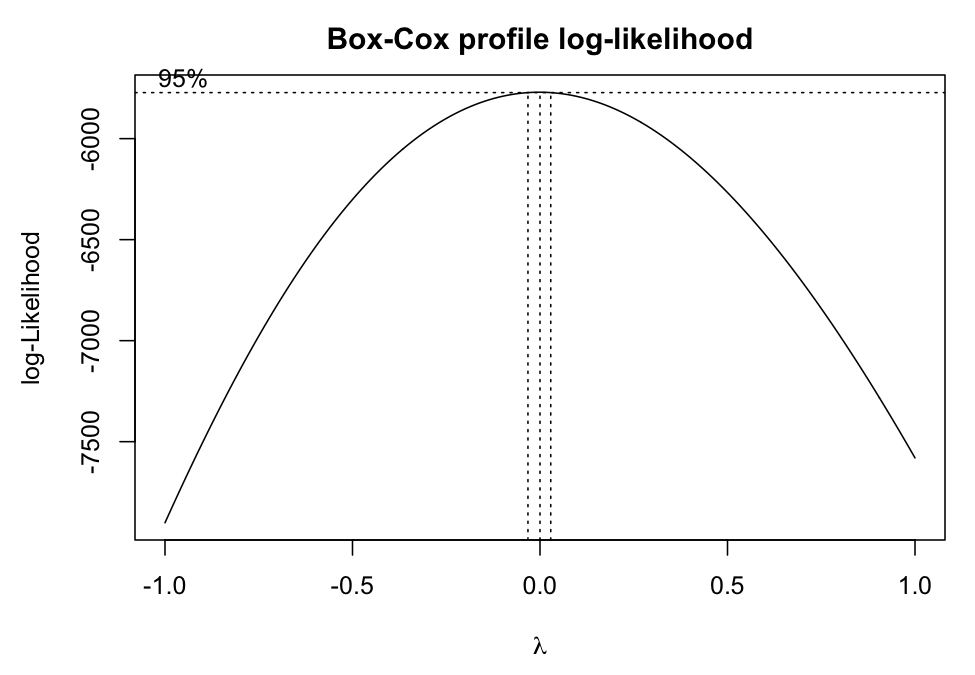
\includegraphics[width=\textwidth]{images/fig4_boxcox.png}
        \captionof{figure}{Box-Cox log-likelihood for market value. The peak is at $\lambda = 0$ (log).}
        \label{fig:boxcox}
    \end{minipage}\hfill
    \begin{minipage}[c]{0.5\textwidth}
        \centering
        \captionof{table}{Correlations among the quantitative predictors.}
        \label{tab:cor}
        \small
        \begin{tabular}{lrrrr}
            \toprule
                    & Age  & G+A/90  & Pass \% & Minutes \\
            \midrule
            Age     & 1.00 & $-0.08$ & $-0.05$ & 0.07    \\
            G+A/90  &      & 1.00    & $-0.09$ & 0.05    \\
            Pass \% &      &         & 1.00    & $-0.01$ \\
            Minutes &      &         &         & 1.00    \\
            \bottomrule
        \end{tabular}
    \end{minipage}
\end{figure}

\subsection*{A.7 Simple linear regressions}
Table~\ref{tab:slr} shows simple regressions of market value (in millions) on each predictor. G+A/90 is the strongest predictor (slope $= 40.84$, $t = 24.46$, $p < 0.001$, $R^2 = 0.268$): 0.1 more G+A per 90 goes with about \euro4.1M more value. The other predictors are significant but explain little ($R^2 \le 0.087$). The residual plots (Figure~\ref{fig:slr}) show three problems in all four models: the residual spread grows with the fitted values, the residuals are right-skewed, and the age relationship is curved.

\begin{table}[!htb]
    \centering
    \caption{Simple linear regressions of market value (millions) on each predictor ($n = 1{,}638$).}
    \label{tab:slr}
    \small
    \begin{tabular}{lrrrrr}
        \toprule
        Predictor            & Slope    & SE     & $t$     & $p$       & $R^2$ \\
        \midrule
        Age (years)          & $-0.729$ & 0.107  & $-6.80$ & $< 0.001$ & 0.028 \\
        G+A per 90           & 40.84    & 1.670  & 24.46   & $< 0.001$ & 0.268 \\
        Pass completion (\%) & 0.403    & 0.051  & 7.86    & $< 0.001$ & 0.036 \\
        Minutes played       & 0.0067   & 0.0005 & 12.46   & $< 0.001$ & 0.087 \\
        \bottomrule
    \end{tabular}
\end{table}

\begin{figure}[!htb]
    \centering
    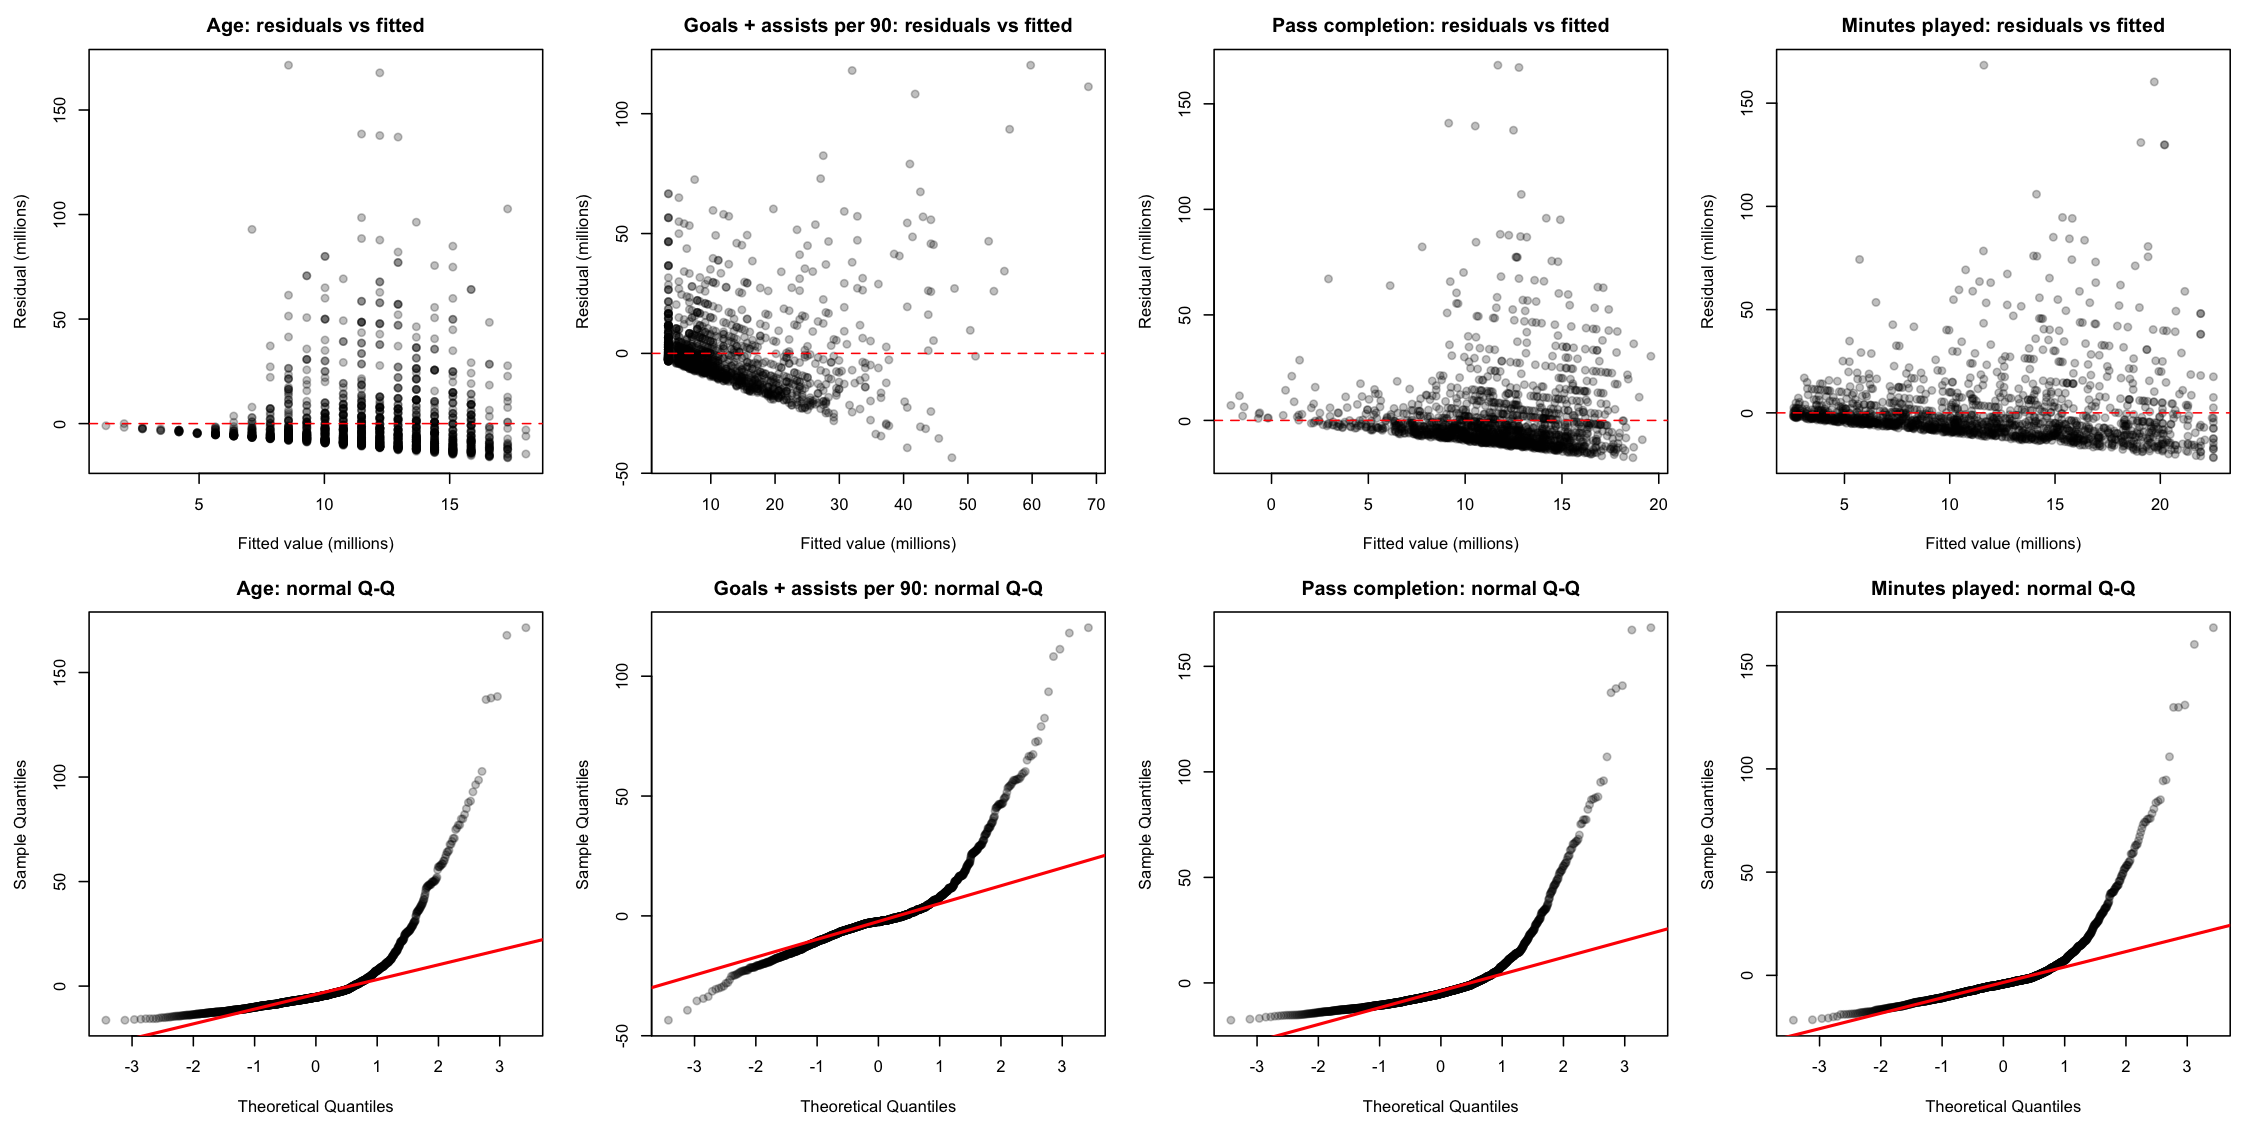
\includegraphics[width=0.88\textwidth]{images/fig3_slr_diagnostics.png}
    \caption{Residuals versus fitted values (top) and normal Q-Q plots (bottom) for the four simple regressions.}
    \label{fig:slr}
\end{figure}

\subsection*{A.8 Proposed remedies}
\begin{enumerate}
    \item Use log(market value) as the response, as Box-Cox suggests. This also evens out the residual spread.
    \item Add age$^2$ and (pass \%)$^2$ to capture the curvature.
    \item Keep the star players, but check their influence with Cook's distance in Part B.
\end{enumerate}

\clearpage
\section*{Part B: Deeper analysis and preliminary conclusions}

\subsection*{B.1 Candidate multiple regression models}
We built the model in steps and tested each added term with a partial $F$-test (Table~\ref{tab:models}). Every model includes all five predictors, with DF as the baseline position.
\begin{itemize}
    \item \textbf{M1:} market value on the five predictors.
    \item \textbf{M2:} the same model for log(market value).
    \item \textbf{M3:} M2 plus age$^2$.
    \item \textbf{M4:} M3 plus (pass \%)$^2$.
\end{itemize}
Switching to log(value) fixed the main residual problems (Figure~\ref{fig:diag}). Adding age$^2$ ($F = 108.27$, $p < 0.001$) and then (pass \%)$^2$ ($F = 75.99$, $p < 0.001$) both improved the fit, raising adjusted $R^2$ from 0.544 to 0.591. We also tried letting the effects of G+A/90 and pass completion differ by position (interaction terms), but neither helped ($p = 0.822$ and $p = 0.370$). We therefore choose \textbf{M4}.

\begin{table}[!htb]
    \centering
    \caption{Candidate models. The partial $F$-test compares each model with the one before it. M1's $R^2$ is for the original value scale, so it is not directly comparable with the others.}
    \label{tab:models}
    \small
    \begin{tabular}{lllrrl}
        \toprule
        Model       & Response   & Predictors                & $R^2$ & Adj.\ $R^2$ & Partial $F$-test          \\
        \midrule
        M1          & value      & main effects              & 0.451 & 0.449       & ---                       \\
        M2          & log(value) & main effects              & 0.546 & 0.544       & ---                       \\
        M3          & log(value) & + age$^2$                 & 0.574 & 0.572       & $F = 108.27$, $p < 0.001$ \\
        \textbf{M4} & log(value) & + age$^2$ + (pass \%)$^2$ & 0.593 & 0.591       & $F = 75.99$, $p < 0.001$  \\
        \bottomrule
    \end{tabular}
\end{table}

\textbf{Checking assumptions.} For M4, the residuals have roughly constant spread and the normal Q-Q plot is close to a straight line, unlike M1 (Figure~\ref{fig:diag}). No player has a large Cook's distance (largest 0.023). Refitting without the 80 players with Cook's distance above $4/n$ gives similar coefficients. The only change is that the midfielder vs.\ defender difference becomes significant ($p = 0.010$), so we interpret that comparison with caution.

\begin{figure}[!htb]
    \centering
    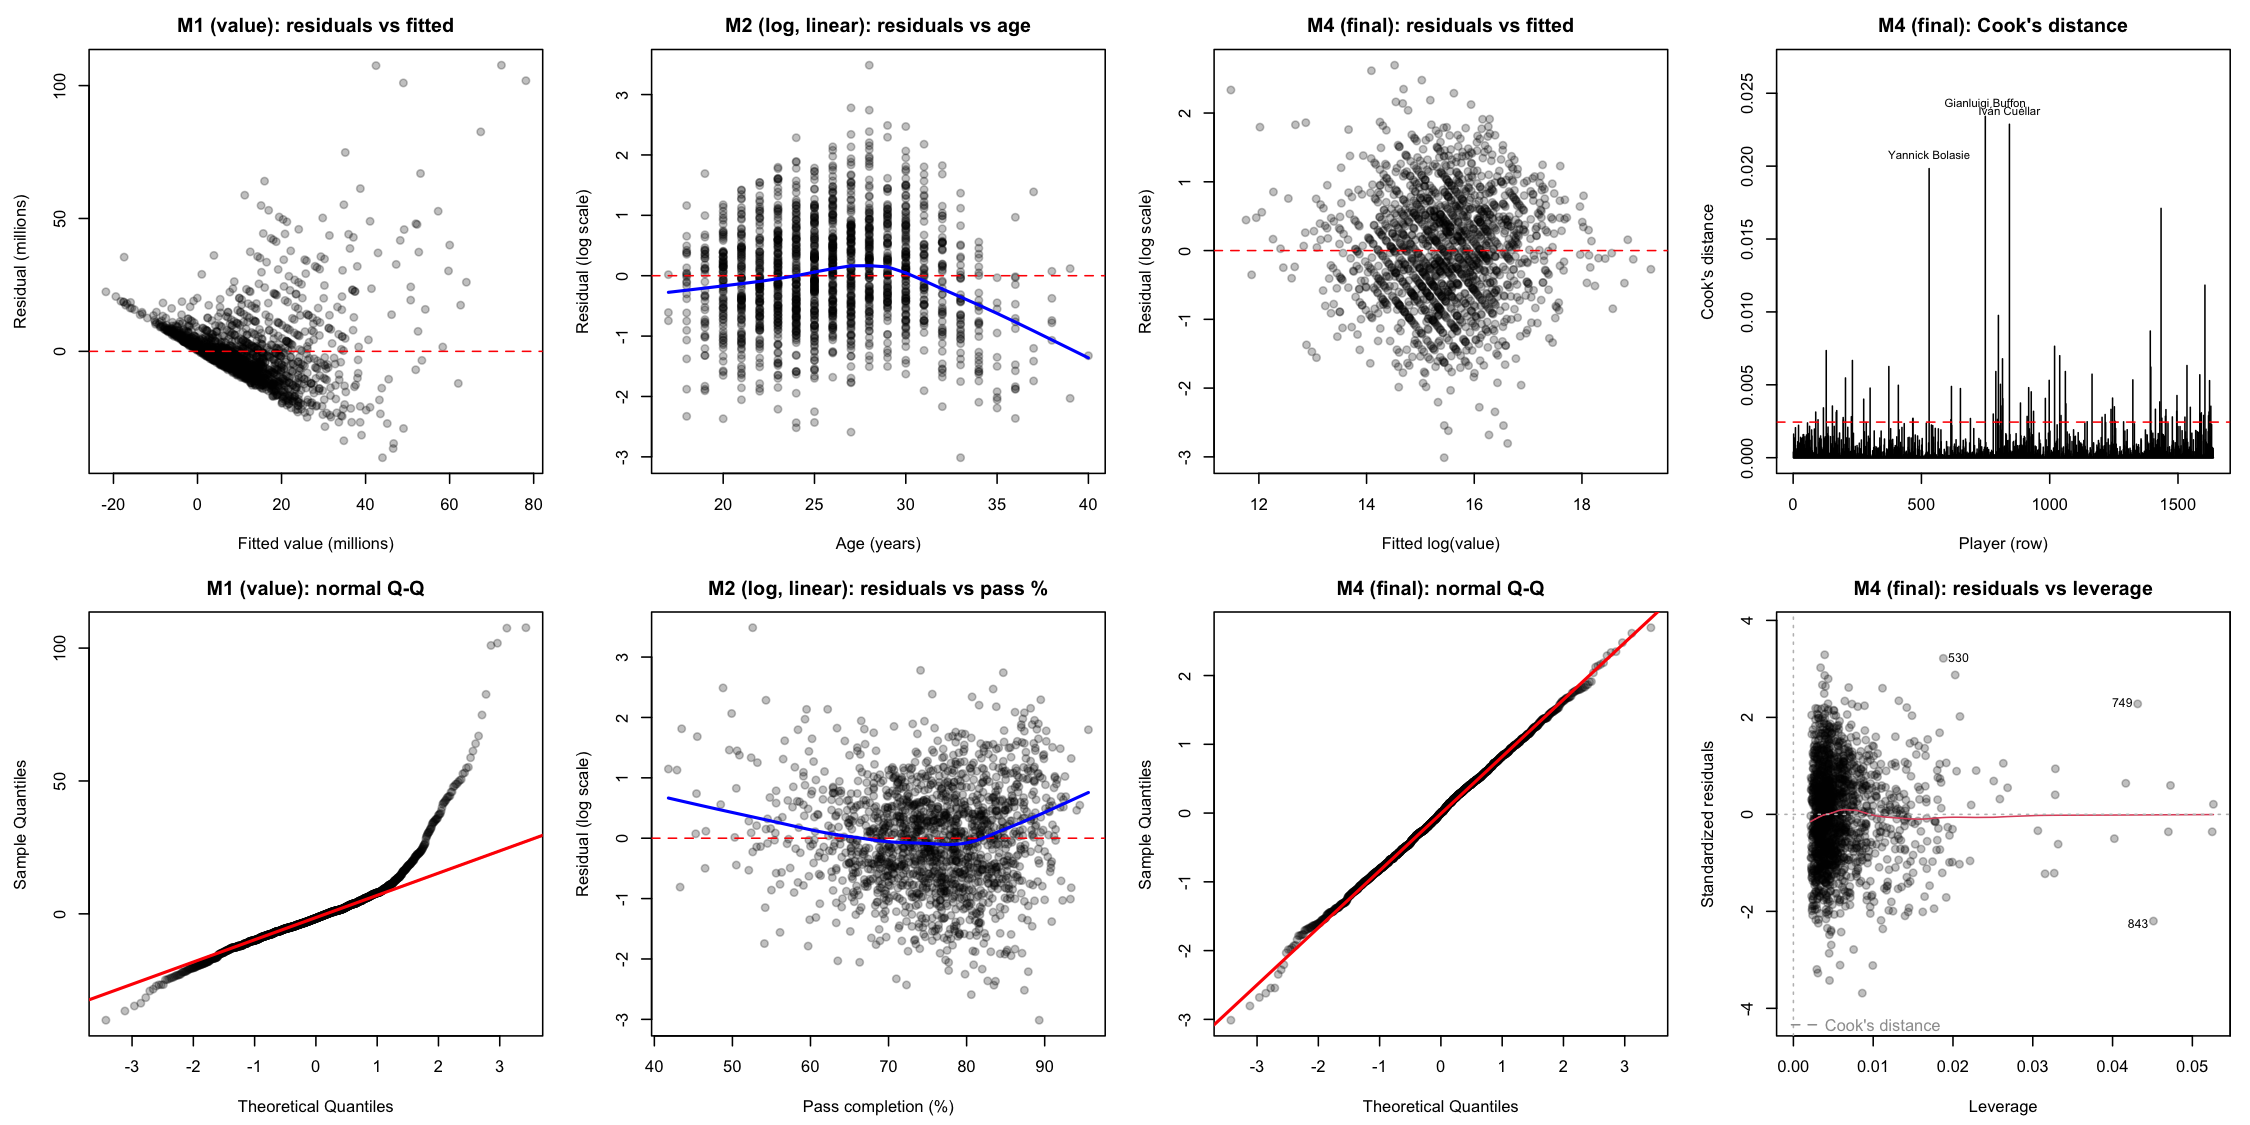
\includegraphics[width=\textwidth]{images/fig5_model_diagnostics.png}
    \caption{Model diagnostics. Column 1: M1 (raw value) has fanning, right-skewed residuals. Column 2: residuals of M2 against age and pass completion are curved (blue trend lines), which motivates the squared terms. Columns 3--4: the final model M4 has even, roughly normal residuals and no highly influential players.}
    \label{fig:diag}
\end{figure}

\subsection*{B.2 Key findings and interpretation}
M4 explains 59\% of the variation in log market value (adjusted $R^2 = 0.591$). Because the response is log(value), a coefficient $b$ means roughly a $100(e^{b} - 1)\%$ change in market value for a one-unit increase in that predictor, holding the others fixed (Table~\ref{tab:coef}).

\begin{table}[!htb]
    \centering
    \caption{Final model M4 for log(market value). Age and pass completion are centered at their means (25.9 years and 75.7\%); DF is the baseline position.}
    \label{tab:coef}
    \small
    \begin{tabular}{lrrrrl}
        \toprule
        Term               & Estimate  & SE       & $t$      & $p$       & Meaning                     \\
        \midrule
        Intercept          & 14.00     & 0.0648   & 216.18   & $< 0.001$ &                             \\
        Age (centered)     & $-0.1025$ & 0.0052   & $-19.74$ & $< 0.001$ & value peaks near age 21     \\
        Age$^2$            & $-0.0102$ & 0.0010   & $-10.58$ & $< 0.001$ &                             \\
        G+A per 90         & 2.653     & 0.1195   & 22.21    & $< 0.001$ & $+30\%$ per extra 0.1       \\
        Pass \% (centered) & 0.0554    & 0.0029   & 19.00    & $< 0.001$ &                             \\
        Pass \%$^2$        & 0.00174   & 0.00020  & 8.72     & $< 0.001$ &                             \\
        Minutes            & 0.000556  & 0.000027 & 20.62    & $< 0.001$ & $+5\%$ per extra 90 minutes \\
        MF (vs DF)         & $-0.0893$ & 0.0509   & $-1.75$  & 0.079     & $-8.5\%$ (not significant)  \\
        FW (vs DF)         & $-0.0598$ & 0.0720   & $-0.83$  & 0.407     & $-5.8\%$ (not significant)  \\
        GK (vs DF)         & 0.5341    & 0.1026   & 5.21     & $< 0.001$ & $+71\%$                     \\
        \bottomrule
    \end{tabular}
\end{table}

The examples below are predicted values for a typical player at that position (Figure~\ref{fig:effects}).
\begin{itemize}
    \item \textbf{Goals + assists} is the strongest predictor ($b = 2.653$, $t = 22.21$, $p < 0.001$). Each extra 0.1 G+A per 90 minutes goes with about 30\% higher value: a typical forward is worth \euro3.3M with 0.1 G+A/90 and \euro9.4M with 0.5.
    \item \textbf{Minutes played:} each extra 90 minutes goes with about 5\% higher value ($b = 0.000556$, $t = 20.62$, $p < 0.001$). A typical midfielder is worth \euro3.6M with 900 minutes and \euro9.7M with 2{,}700.
    \item \textbf{Age:} value peaks near age 21 and then falls faster each year. A typical midfielder is worth \euro6.7M at 22, \euro4.0M at 28 and \euro2.4M at 31.
    \item \textbf{Pass completion:} higher is better, especially at the top end. A typical midfielder is worth \euro3.1M at 65\%, \euro4.5M at 75\% and \euro9.0M at 85\%.
    \item \textbf{Position:} with the same statistics, goalkeepers are worth about 71\% more than defenders ($p < 0.001$), because keepers are not expected to score or assist. Midfielders and forwards do not differ significantly from defenders.
\end{itemize}

\begin{figure}[!htb]
    \centering
    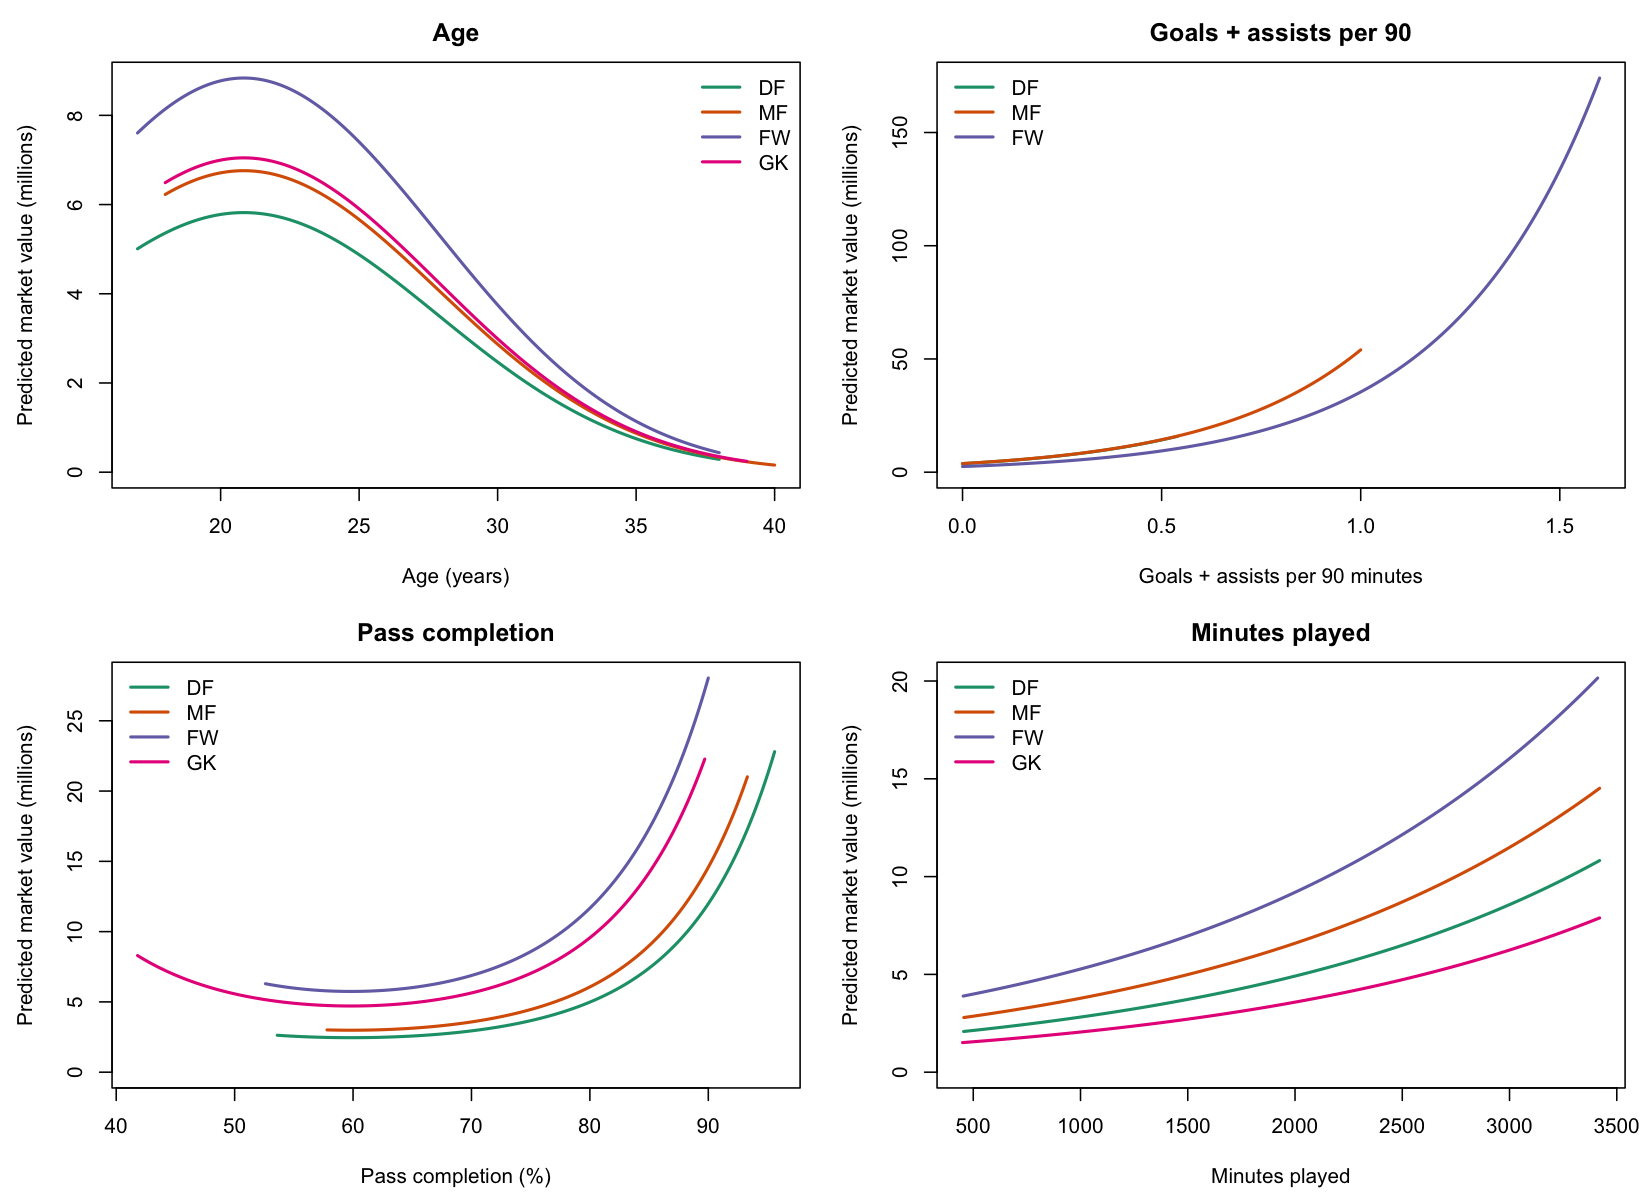
\includegraphics[width=0.8\textwidth]{images/fig6_effects.png}
    \caption{Predicted market value from M4 as each predictor changes, for a typical player at each position (other predictors at that position's medians).}
    \label{fig:effects}
\end{figure}

\textbf{Preliminary conclusions.} Players who score or assist more, play more minutes, pass more accurately and are younger tend to have higher market values. Together these factors explain about 60\% of the variation in log market value. These are associations, not causes, and other factors such as league, club and contract length are not in our data. For the final report we plan to check the $\times10$ correction against Transfermarkt and test the model on the 2018/19 season.

\vspace{0.5em}
{\small\textbf{Code.} \texttt{prepare\_data.R} (cleaning), \texttt{make\_figures.R} (Part A), \texttt{part2\_models.R} (Part B). AI was used for a small part of cleaning the data, as well as formatting for this PDF progress report.

    \textbf{References}\\
    {[1]} Kaggle user kriegsmaschine. \emph{Soccer players values and their statistics} (transfermarkt.de and fbref.com merged data, 2017/18--2019/20).\\ \url{https://www.kaggle.com/datasets/kriegsmaschine/soccer-players-values-and-their-statistics}}

\end{document}
